\section{Dimensioning}

The dimensioning process involves optimizing the Recycling Folded-Cascode (RFC) OTA design to achieve the specified performance goals while adhering to the given constraints. Hence, a python script was created according to the analysis made in section \ref{sec:TheoreticalAnalysys}. This script showed how varying different parameters affected the circuit behavior and calculated the size of all transistors respecting size ratios. 

In order to have a more modular script three dictionaries were created to save all transistors characteristics and a list with all transistors names making the list iterable.

As a starting point all transistors sizes were set to have length of $\SI{600}{\nano\meter}$ and a $V_{DSsat} = \SI{100}{\milli\volt}$, to ensure the devices were operating in the moderate inversion region, as specified in Table \ref{tab:goals}. Then the gain equation was analyzed in order to find the transistors affected this value.

\subsection{DC gain analysis}
\label{sec:DCGain}
In order to achieve the DC gain goal of $\SI{66}{\decibel}$, it is important to first identify the devices that will influence this value and specifically what parameters. \textcolor{red}{Faltam coisas aqui ver comment}

%TODO REF NA EQUACAO DO GANHO
%Table \ref{tab:GainTransistors}, shows the devices characteristics that affect gain, this was done by analysing \ref{eq:AvFinal}.

\begin{table}[H]
    \centering
    \caption{Transistor's characteristics that affect gain}
    \begin{tabularx}{\textwidth}{>{\centering\arraybackslash}X >{\centering\arraybackslash}X >{\centering\arraybackslash}X}
        \toprule
        \textbf{Transistor} & \textbf{$V_{DSsat}$} & \textbf{$L_{size}$} \\
        \midrule
        $M_{3}$ & $\checkmark$ & $\checkmark$\\
        \midrule
        $M_{2a}$ & $\checkmark$ & $\times$\\
        \midrule
        $M_{1b}$ & $\checkmark$ & $\times$\\
        \midrule
        $M_{5}$ & $\checkmark$ & $\checkmark$\\
        \midrule
        $M_{11}$ & $\times$ & $\checkmark$\\
        \midrule
        $M_{7a}$ & $\times$ & $\checkmark$\\
        \bottomrule
    \end{tabularx}
    \label{tab:GainTransistors}
\end{table}

To visualize how each parameter influence the gain value independently, the gain function was plotted varying one parameter at a time, creating the graphs shown in Figure \ref{fig:GainVariation}. 

\begin{figure}[H]
    \centering
    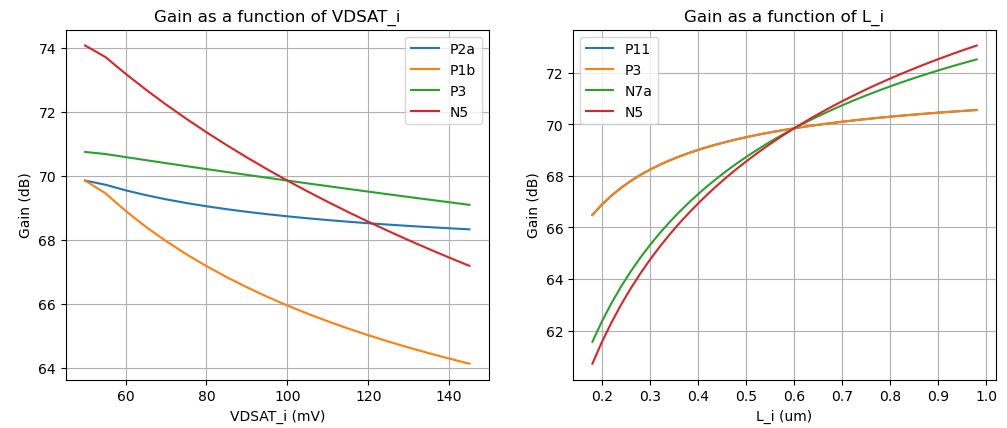
\includegraphics[width=1\textwidth]{Images/GainVariation.png}
    \caption{Gain as a function of $V_{DSsat}$ and $L_{size}$}
    \label{fig:GainVariation}
\end{figure}

As shown by Figure \ref{fig:GainVariation}, the parameters that are more relevant are, $M_{5}$ and $M_{1b}$ $V_{DSsat}$ and $M_{5}$ and $M_{7a}$ length size.

Knowing this, a heatmap was plotted, Figure \ref{fig:GainHeatMap}. The heatmap provides a more complete picture by displaying the combined influence of both variables on the gain function. Each cell in the heatmap corresponds to a specific pair of values for the two variables, with the color intensity indicating the resulting gain.

\begin{figure}[H]
    \centering
    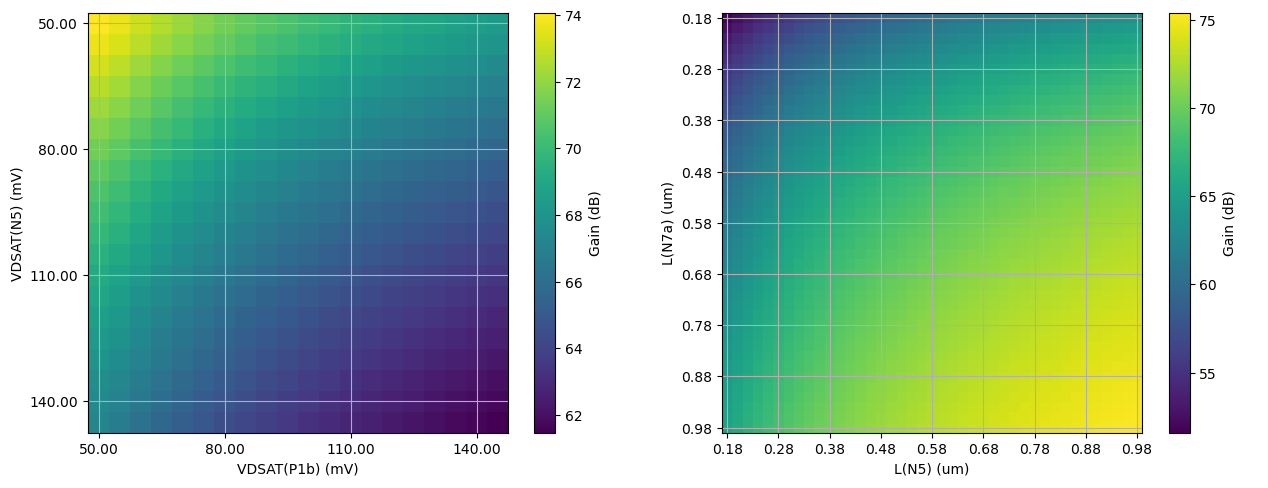
\includegraphics[width=1\textwidth]{Images/GainHeatMap.png}
    \caption{Gain HeatMap}
    \label{fig:GainHeatMap}
\end{figure}


\subsection{Gain Bandwidth Product (GBW) analysis}
\label{sec:GBWPython}
Analogously to the subsection \ref{sec:DCGain}, to achieve the Gain Bandwidth Product (GBW) target of $\SI{100}{\mega\hertz}$, the devices and parameters that influence this performance metric must be identified.\textcolor{red}{Faltam coisas aqui ver comment}

%TODO REF NA EQUACAO DO GANHO
%Using equation \ref{eq:GBW}, the table \ref{tab:GBWTransistors} was constructed.

\begin{table}[h]
    \centering
    \caption{Transistor's characteristics that affect gain}
    \begin{tabularx}{\textwidth}{>{\centering\arraybackslash}X >{\centering\arraybackslash}X >{\centering\arraybackslash}X}
        \toprule
        \textbf{Transistor} & \textbf{$V_{DSsat}$} & \textbf{$L_{size}$} \\
        \midrule
        $M_{3}$ & $\checkmark$ & $\checkmark$\\
        \midrule
        $M_{2a}$ & $\checkmark$ & $\times$\\
        \midrule
        $M_{1b}$ & $\checkmark$ & $\times$\\
        \midrule
        $M_{5}$ & $\checkmark$ & $\checkmark$\\
        \bottomrule
    \end{tabularx}
    \label{tab:GBWTransistors}
\end{table}

Again to visualize how each parameter influence the GBW independently, the GBW function was plotted varying each parameter at a time, yielding Figure \ref{fig:GBWVariation}.

\begin{figure}[H]
    \centering
    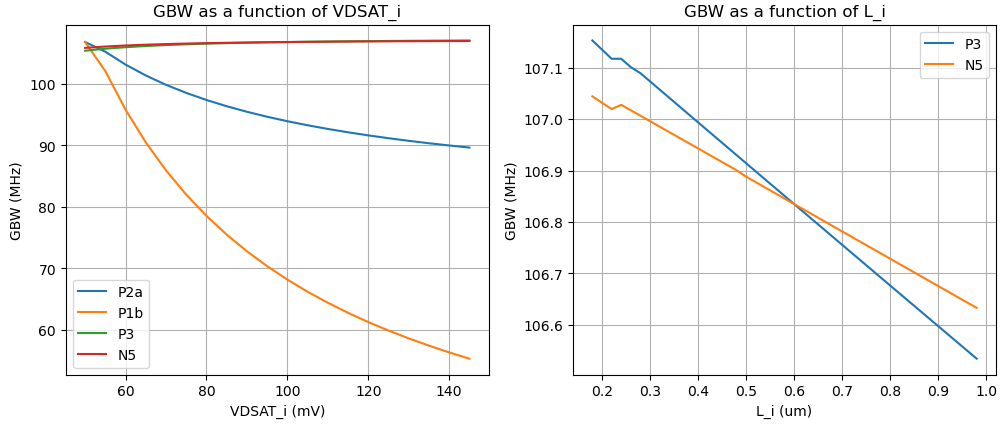
\includegraphics[width=1\textwidth]{Images/GBWVariation.png}
    \caption{GBW as a function of $V_{DSsat}$ and $L_{size}$}
    \label{fig:GBWVariation}
\end{figure}

Because for $V_{DSsat}$, devices $M_{1b}$ and $M_{2a}$ change the GBW value more drastically and for $L_{size}$ there are only two devices that affect the final value, a heatmap was plotted, yielding Figure \ref{fig:GBWHeatMap}. 

\begin{figure}[H]
    \centering
    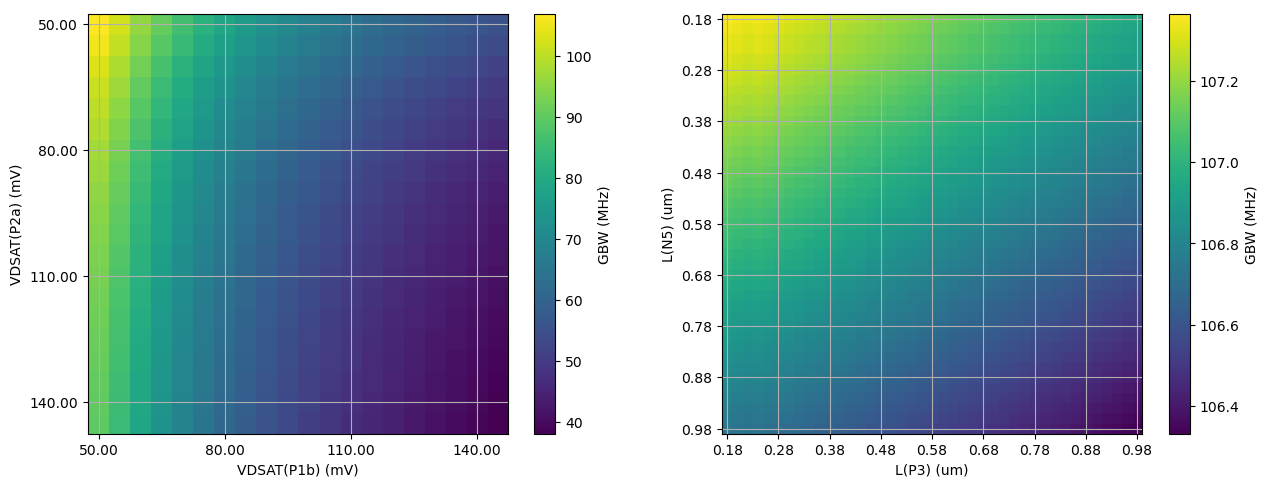
\includegraphics[width=1\textwidth]{Images/GBWHeatMap.png}
    \caption{GBW HeatMap}
    \label{fig:GBWHeatMap}
\end{figure}

\subsection{Pole Frequencies analysis}

Because almost all poles depend on the $V_{DSsat}$ and $L_{size}$ of all devices that appear in its equation, there was no distinction made between the devices in the $V_{DSsat}$ an $L_{size}$ plots.

\textcolor{red}{PAO sq dizer cena da estabilidade e cena da ordem}

\begin{figure}[H]
    \centering
    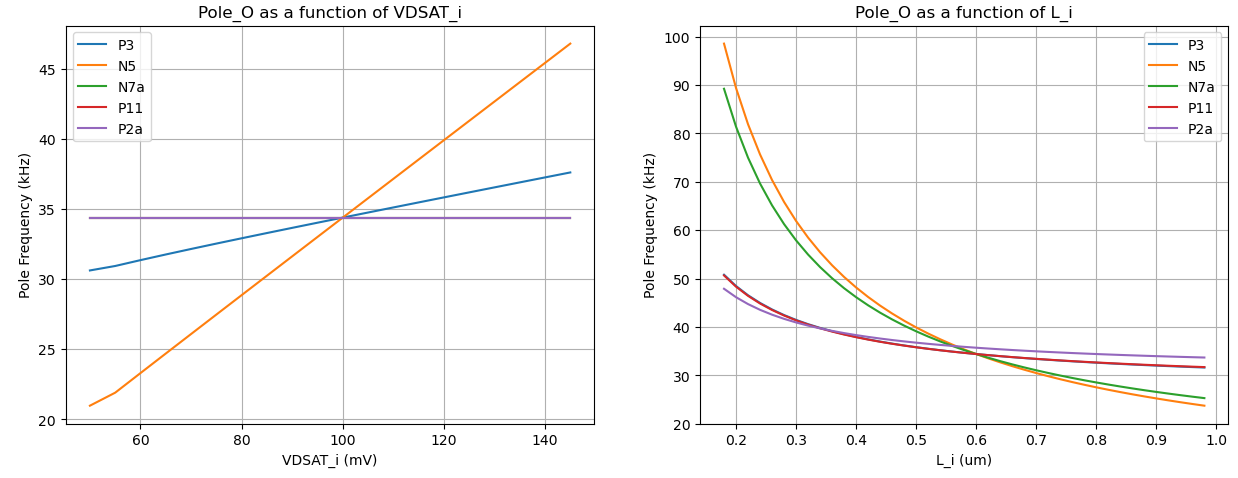
\includegraphics[width=1\textwidth]{Images/PoPlot.png}
    \caption{Output Pole as a function of $V_{DSsat}$ and $L_{size}$}
    \label{fig:PoPlot}
\end{figure}

For the first it is the least relevant, since it only affects GBW and that parameter was already explored in section \ref{sec:GBWPython}.

\begin{figure}[H]
    \centering
    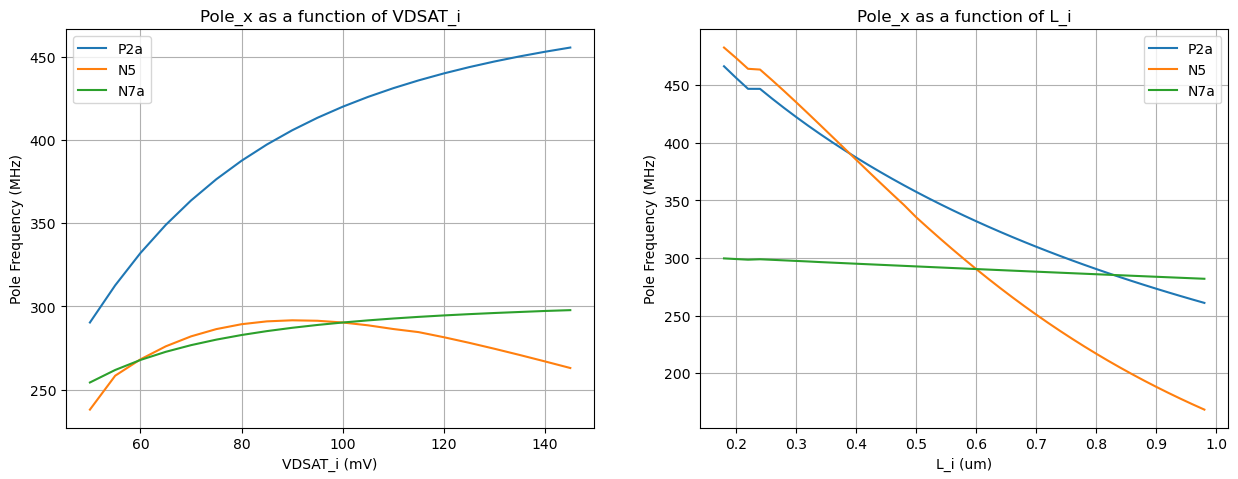
\includegraphics[width=1\textwidth]{Images/PxPlot.png}
    \caption{Pole $x$ as a function of $V_{DSsat}$ and $L_{size}$}
    \label{fig:PxPlot}
\end{figure}

\begin{figure}[H]
    \centering
    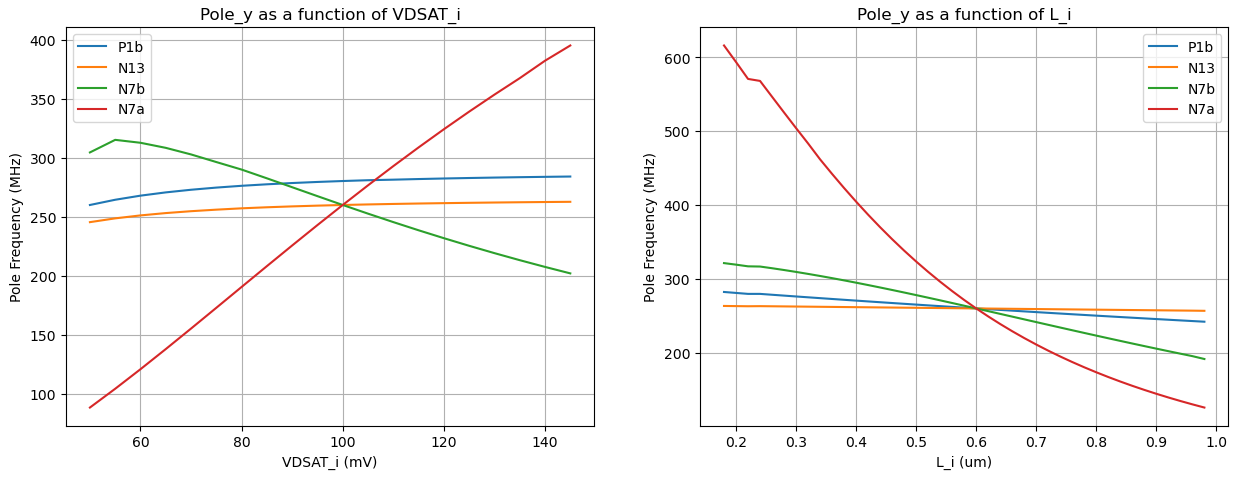
\includegraphics[width=1\textwidth]{Images/PyPlot.png}
    \caption{Pole $y$ as a function of $V_{DSsat}$ and $L_{size}$}
    \label{fig:PyPlot}
\end{figure}

\begin{figure}[H]
    \centering
    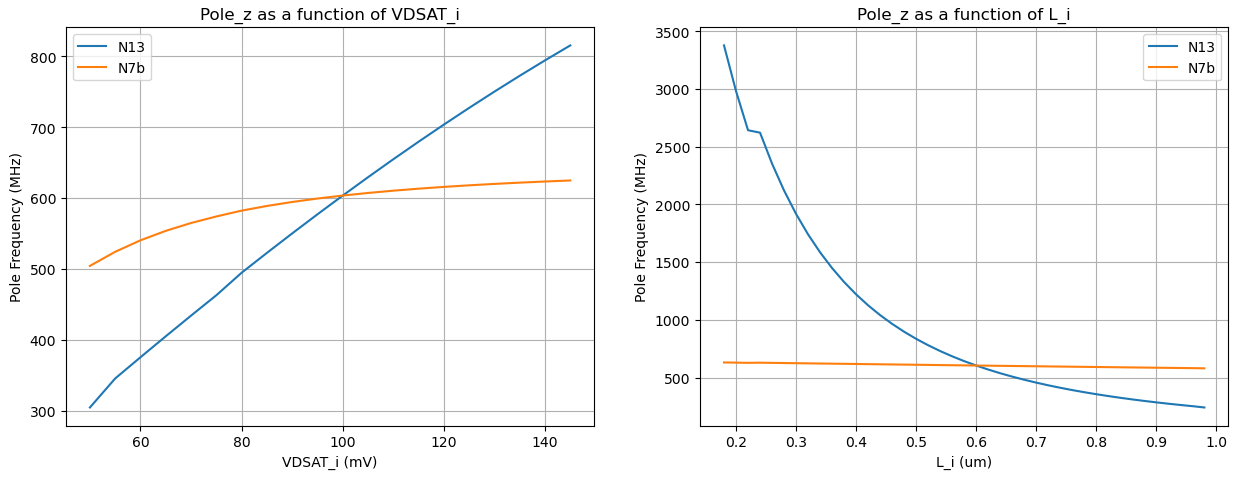
\includegraphics[width=1\textwidth]{Images/PzPlot.png}
    \caption{Pole $z$ as a function of $V_{DSsat}$ and $L_{size}$}
    \label{fig:PzPlot}
\end{figure}

\begin{figure}[H]
    \centering
    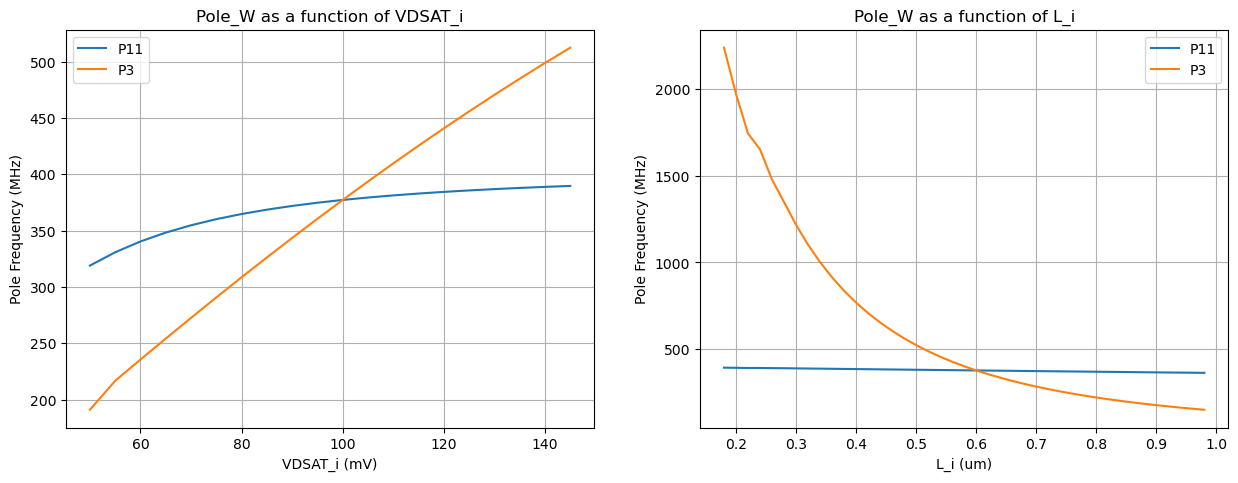
\includegraphics[width=1\textwidth]{Images/PwPlot.png}
    \caption{Pole $w$ as a function of $V_{DSsat}$ and $L_{size}$}
    \label{fig:PwPlot}
\end{figure}




\subsection{Output Swing (OS) analysis}

\subsection{Excess-Noise Factor (ENF) analysis}

\subsection{Power Consumption analysis}

\subsection{Merit Figure and Results}
